\section{Introduction}
\label{sec:introduction}

Repetitive motion is a useful measurement primitive. Exercise coaching,
rehabilitation, industrial monitoring, sports analysis, and human--robot
interaction all require more than recognizing that an action repeats: a
system must determine how often each participant repeats it. In an
uncontrolled scene, however, people need not move together. One person may
slow down while another accelerates, a third may pause, and tracks may contain
gaps caused by occlusion. A single response curve for the whole frame can
therefore mix identities and incompatible time scales, producing a plausible
scene total while assigning the wrong count to each person.

Repetition counting has progressed from online local cycle
estimation~\cite{levy2015live} and motion-frequency
analysis~\cite{runia2018realworld} to learned
temporal self-similarity, density regression, and dynamic-query models
~\cite{dwibedi2020repnet,hu2022transrac,ma2026detrc}. ESCounts studies
exemplar-conditioned counting and predicts one target density/count stream
~\cite{sinha2024escounts}. SkimFocusNet studies exemplar-selected multiple
action types~\cite{zhao2025skimfocus}. These advances largely assume one
counted stream. MultiCounter formalizes multi-instance repetitive action
counting and jointly predicts people, identities, periodic intervals, and
counts~\cite{tang2024multicounter}; MultiCounter+ strengthens temporal identity
consistency and long/short-period awareness~\cite{tang2026multicounterplus}.
Consequently, multi-person, person-wise, asynchronous, and variable-speed
counting are established problems rather than novelty claims of this paper.

The remaining opportunity lies at the intersection of supervision, modality,
and temporal granularity. Existing MRAC systems are trained as supervised RGB
pipelines, whereas pose-based and label-efficient counting has been developed
mostly for a single instance. PoseRAC exploits salient poses in an open-set,
zero-shot framework~\cite{yao2025poserac}; D$^2$-STX combines RGB and pose
streams~\cite{wang2026d2stx}; and PAMS learns pose representations through
period-adaptive multi-scale consistency without repetition annotations
~\cite{gao2026pams}. PAMS also evaluates robustness under uniform global speed
resampling, but it does not separate simultaneous identities. Conversely, MRAC
identity mechanisms do
not directly provide an annotation-efficient, pose-driven counter whose tempo
assignment can change from window to window along one person's track.

We study that constrained setting. An upstream perception system supplies
identity-indexed pose tracks and validity masks. The counting model shares its
encoder and tempo experts across people, but maintains independent buffers,
routing weights, and output streams for each identity. A masked local period
estimate selects a soft mixture of fast, medium, and slow experts within every
overlapping window. Instead of counting windows and adding their integer
outputs, the model stitches continuous responses with normalized overlap-add
and performs one final peak extraction per track. This ordering makes the
window boundary explicit and removes the direct arithmetic path by which one
repetition can be independently counted in two overlapping windows; it does
not guarantee immunity to phase-misaligned responses.

Figure~\ref{fig:task_comparison} contrasts the target output with a mixed
single-stream counter. The formulation does not assume that tracking errors
have been solved: predicted-track experiments must expose their effect, while
oracle-track experiments isolate the counting module. It also does not call
the whole system free of all labels. A detector, pose estimator, tracker, or
backbone may have external supervision; the narrower intended property is that
the counting objective consumes no person-wise repetition count or period
labels.

\begin{figure*}[t]
  \centering
  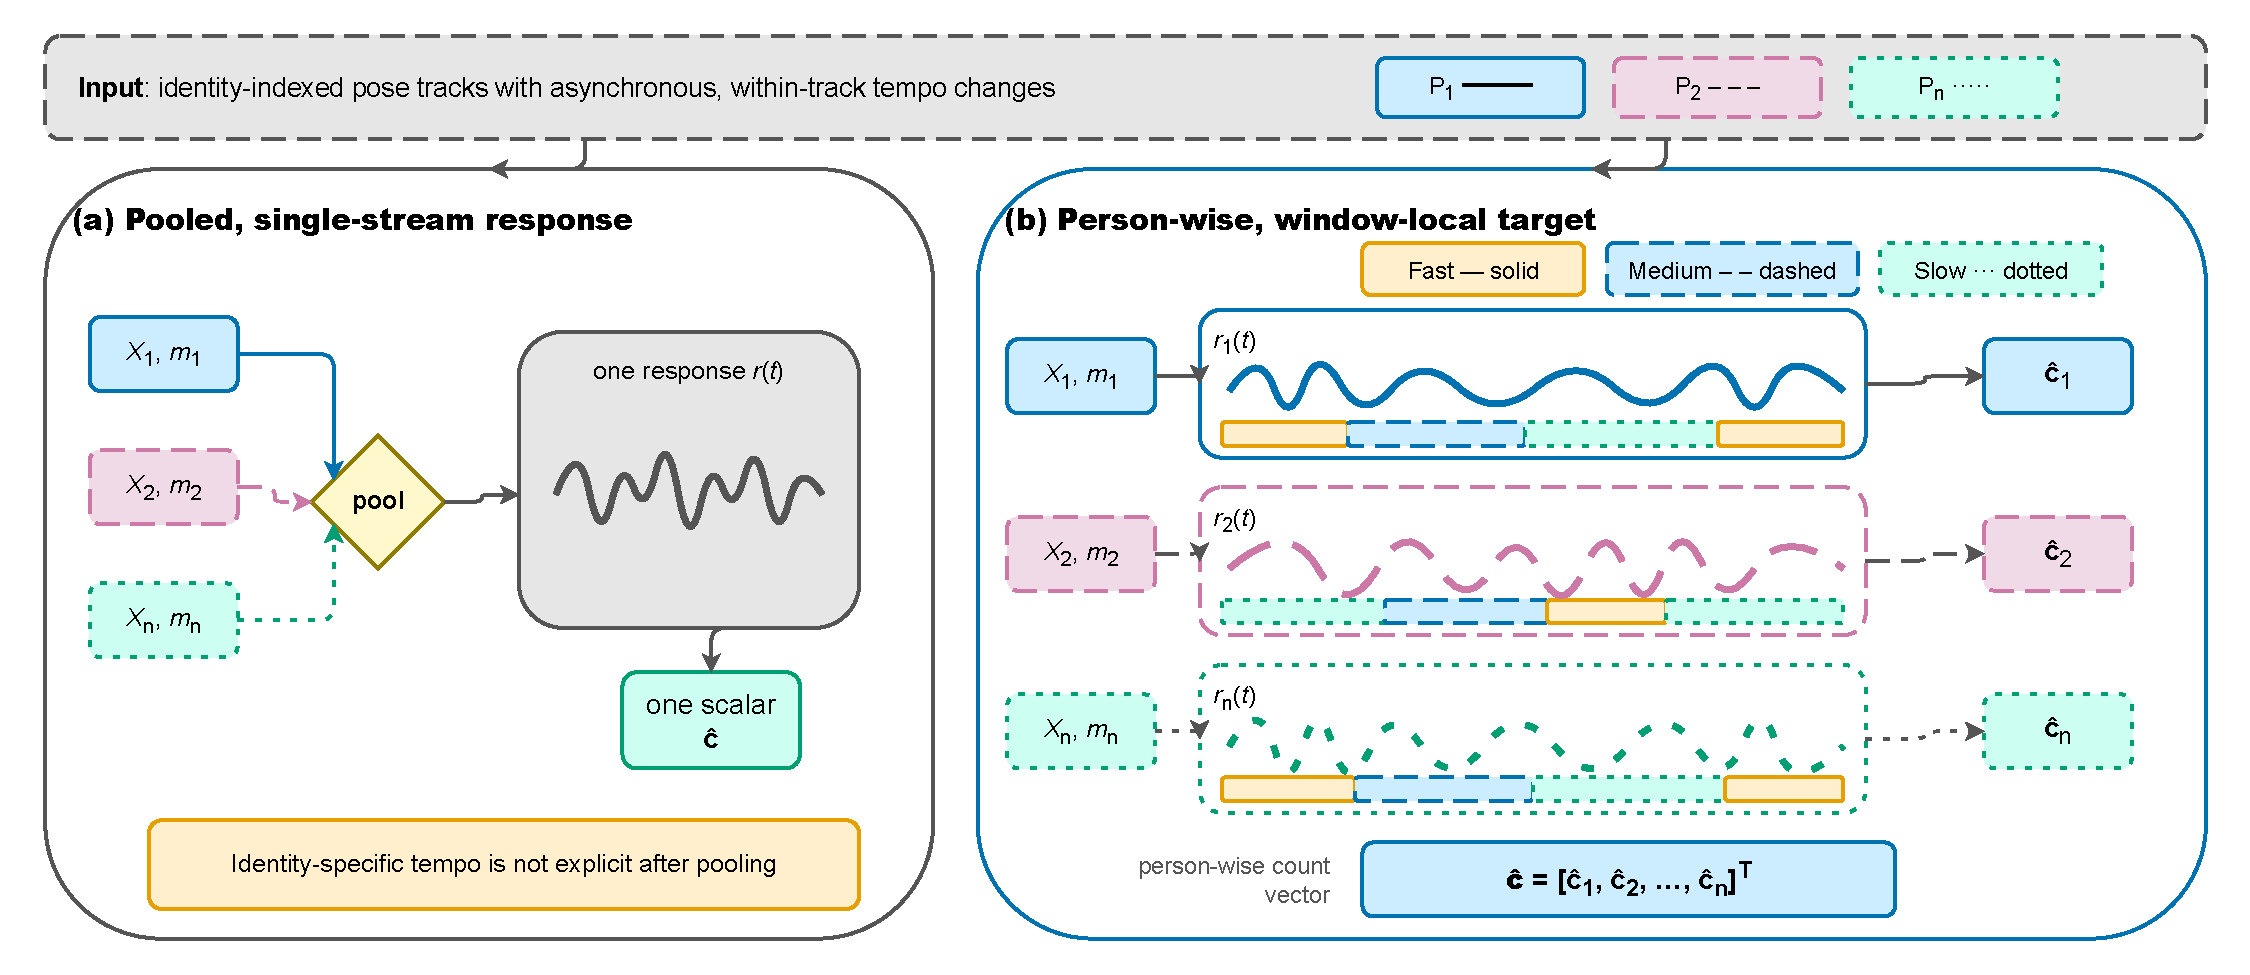
\includegraphics[width=0.98\textwidth]{figures/task_comparison.pdf}
  \caption{\textbf{Target task and output.} The left panel is a naïve pooled
  single-stream failure mode, not MultiCounter or MultiCounter+. A frame-level response can mix
  people who move at different and changing rates (left). We instead retain
  identity-indexed masked pose tracks, estimate tempo locally within each
  track, and return a person-wise count vector (right). The scene total is only
  a derived diagnostic. This is a problem illustration, not result evidence.}
  \label{fig:task_comparison}
\end{figure*}

The paper makes three falsifiable, currently evidence-gated contributions:

\begin{itemize}
  \item \ClaimMap{C01,C02}We formulate a pose-driven MRAC training setting whose intended
  counting loss uses no person-wise count or period annotations, while
  explicitly accounting for externally supervised perception components.
  This supervision statement must be verified against the frozen training
  graph before submission.

  \item \ClaimMap{C03,C04,C05,C06}We propose track-indexed, window-level tempo routing with
  shared parameters and per-track state, followed by response-domain
  overlap-add and one track-level decoding pass. Its benefit must be separated
  from the effects of tracking and the PAMS representation through controlled
  ablations.

  \item \ClaimMap{C10,C12,C15}We establish an evaluation contract that pairs the official MultiRep
  counting metrics with oracle/predicted-track protocols, tracking
  diagnostics, non-stationary-tempo stress tests, and person-count scaling.
  Every final table cell must be generated from a frozen result manifest.
\end{itemize}

This pre-results draft freezes the scientific story and its evidence
requirements; it does not assert that the multi-person modules are already
implemented or that the proposed method outperforms any baseline.
